\documentclass[11pt]{report}
\usepackage{graphicx}

\begin{document}
\begin{titlepage}
	\centering
	{\scshape\LARGE Universita della Svizzera Italiana\par}
		\vspace{0.5cm}

	{\scshape Science of Informatics\par}
	\vspace{1cm}
	{\scshape\Large Bachelor project plan\par}
	\vspace{1.5cm}
	{\huge\bfseries Design Interactive Display Applications for Active and Walk-by Contact Personalization\par}
	\vspace{2cm}
	{\Large\itshape Francesco Saverio Zuppichini\par}
	\vfill
	Supervised by\par
	Marc Langheinric and
	Ivan Elhart
	\vfill

	{\large \today\par}
\end{titlepage}
%\section*{Motivations}
%I always like to work with real time application that must provide a service to the user. More over this project offers me the opportunity to sharp my web skills and to learn a new very used technology such as Django.
%
\section*{Description}
The work in this project will extend the functionality of already existing mobile personalisation framework, called Tacita, in order to support a wider set of web apps and allow for both active and walk-by personalisation. The project aims to develop two web based applications for public displays that will support personalisation through mobile devices. In particular, the work will focus on designing and developing “Public Transportation” and “Upcoming classes” applications. 
\section*{Goal}
Implement two web application, one for smartphone, and one for the displays. Deploy a web server to handle all the connections between the user and the screens in order to show personalised content and store user information such as preferences. 
\section*{Motivation}
I choose this project because it allows me to focus on the design and the software part. The first one is very important, since the two applications are going to be used by real people, and not programmers, they should be provide a friendly and well studied GUI in order to fast understand how to use all the functionalities that my software will provide. Also I will have the opportunity to lean Django, a well know python framework, and to play with the bluetooth beacons.
\section*{Tasks}
\subsection*{Task 1 - Public Transportation App - 3 weeks}
Design and develop a web application using Django development framework to display transport data such as nearby stations and up coming busses by providing and efficient and good looking design optimize for large screen.\\

In detail the web server collects a request from a user and fetch the corresponding information from the opendata.ch public API in order to send them back to the display. 

\subsection*{Task 2 - Supporting Personalisation through Mobile devices - 2 weeks}
Implement an Android App composed by a WebView and a background bluetooth scanning process. 
\\

The web application should provide a interface optimize for small display in order to use the exposed API and to set personal parameters such as colors, icons and avatar.

\subsection*{Task 3 - Integration of personalisation parameters into display app - 2 weeks}
The aim of this task is to link the previously developed Android Application to the Django web in order to provide a way to storing user preferences into the database and to display them in the screen as default one.
\subsection*{Task 4 - Upcoming Classes App: Collecting, Processing, and Visualising data from a Google Calendar - 2 weeks}
Similarly to what we have done with opendata.ch, add a google calendar app to know the schedule for the course.

\subsection*{Task 5 - Testing - 1 week}
Test the developed code, write unit testing for the endpoints and the web applications.
\subsection*{Task 6 - Users Feedback - 2 week}
Present a demo application to a small subset of students in order to collect feedbacks and, if needed, adjust some features.
\subsection*{Task 7 - Final report - 1 week}
Write down the final report
\begin{figure}[h]
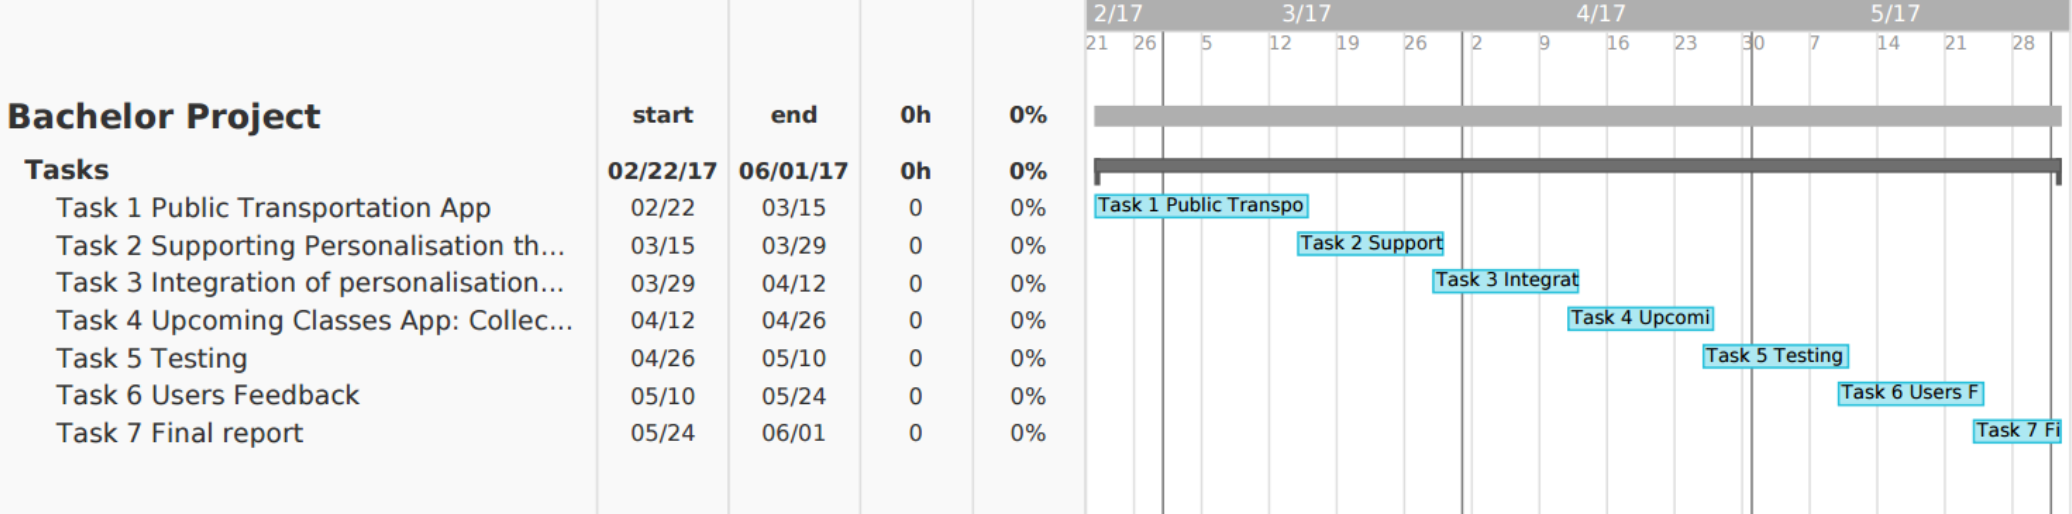
\includegraphics[scale=0.4]{1.png}
\end{figure}
\end{document}



 